%%
%% Copyright 2007, 2008, 2009 Elsevier Ltd
%%
%% This file is part of the 'Elsarticle Bundle'.
%% ---------------------------------------------
%%
%% It may be distributed under the conditions of the LaTeX Project Public
%% License, either version 1.2 of this license or (at your option) any
%% later version.  The latest version of this license is in
%%    http://www.latex-project.org/lppl.txt
%% and version 1.2 or later is part of all distributions of LaTeX
%% version 1999/12/01 or later.
%%
%% The list of all files belonging to the 'Elsarticle Bundle' is
%% given in the file `manifest.txt'.
%%

%% Template article for Elsevier's document class `elsarticle'
%% with harvard style bibliographic references
%% SP 2008/03/01
%%
%%
%%
%% $Id: elsarticle-template-harv.tex 4 2009-10-24 08:22:58Z rishi $
%%
%%
\documentclass[preprint,authoryear,12pt]{elsarticle}

%% Use the option review to obtain double line spacing
%% \documentclass[authoryear,preprint,review,12pt]{elsarticle}

%% Use the options 1p,twocolumn; 3p; 3p,twocolumn; 5p; or 5p,twocolumn
%% for a journal layout:
%% \documentclass[final,authoryear,1p,times]{elsarticle}
%% \documentclass[final,authoryear,1p,times,twocolumn]{elsarticle}
%% \documentclass[final,authoryear,3p,times]{elsarticle}
%% \documentclass[final,authoryear,3p,times,twocolumn]{elsarticle}
%% \documentclass[final,authoryear,5p,times]{elsarticle}
%% \documentclass[final,authoryear,5p,times,twocolumn]{elsarticle}

%% if you use PostScript figures in your article
%% use the graphics package for simple commands
%% \usepackage{graphics}
%% or use the graphicx package for more complicated commands
%% \usepackage{graphicx}
%% or use the epsfig package if you prefer to use the old commands
%% \usepackage{epsfig}

%% The amssymb package provides various useful mathematical symbols
\usepackage{amssymb}
%% The amsthm package provides extended theorem environments
%% \usepackage{amsthm}

%% The lineno packages adds line numbers. Start line numbering with
%% \begin{linenumbers}, end it with \end{linenumbers}. Or switch it on
%% for the whole article with \linenumbers after \end{frontmatter}.
%% \usepackage{lineno}

%% natbib.sty is loaded by default. However, natbib options can be
%% provided with \biboptions{...} command. Following options are
%% valid:

%%   round  -  round parentheses are used (default)
%%   square -  square brackets are used   [option]
%%   curly  -  curly braces are used      {option}
%%   angle  -  angle brackets are used    <option>
%%   semicolon  -  multiple citations separated by semi-colon (default)
%%   colon  - same as semicolon, an earlier confusion
%%   comma  -  separated by comma
%%   authoryear - selects author-year citations (default)
%%   numbers-  selects numerical citations
%%   super  -  numerical citations as superscripts
%%   sort   -  sorts multiple citations according to order in ref. list
%%   sort&compress   -  like sort, but also compresses numerical citations
%%   compress - compresses without sorting
%%   longnamesfirst  -  makes first citation full author list
%%
%% \biboptions{longnamesfirst,comma}

% \biboptions{}

\journal{Transportation Research: Part C}

\begin{document}

\begin{frontmatter}

%% Title, authors and addresses

%% use the tnoteref command within \title for footnotes;
%% use the tnotetext command for the associated footnote;
%% use the fnref command within \author or \address for footnotes;
%% use the fntext command for the associated footnote;
%% use the corref command within \author for corresponding author footnotes;
%% use the cortext command for the associated footnote;
%% use the ead command for the email address,
%% and the form \ead[url] for the home page:
%%
%% \title{Title\tnoteref{label1}}
%% \tnotetext[label1]{}
%% \author{Name\corref{cor1}\fnref{label2}}
%% \ead{email address}
%% \ead[url]{home page}
%% \fntext[label2]{}
%% \cortext[cor1]{}
%% \address{Address\fnref{label3}}
%% \fntext[label3]{}

\title{Articulo requetebonico que queremos que publiquen}

%% use optional labels to link authors explicitly to addresses:
%% \author[label1,label2]{<author name>}
%% \address[label1]{<address>}
%% \address[label2]{<address>}
\author{Muchos y bonitos autores}
\author[uja]{V.M. Rivas\corref{vrivas}}
\ead{vrivas@ujaen.es}
\ead[url]{http://geneura.wordpress.com}
\author[ugr]{M.G. Arenas}
\author[ugr]{P.A. Castillo-Valdivieso}
\address[uja]{Department of Computer Sciences, University of Jaen (Spain)}
\address[ugr]{Department of Architecture and Computer Technology. CITIC. University of Granada (Spain)}
\cortext[vrivas]{Campus Las Lagunillas S/N; E23071, Jaen (Spain)}


\address{}

\begin{abstract}
%% Text of abstract
Blah, blah, blah...
\end{abstract}

\begin{keyword}
%% keywords here, in the form: keyword \sep keyword

%% MSC codes here, in the form: \MSC code \sep code
%% or \MSC[2008] code \sep code (2000 is the default)

\end{keyword}

\end{frontmatter}

% \linenumbers

%% main text
\section{Introduction}
\label{sec:introduction}
The development of new systems of traffic conditions information and the affluence of vehicles on roads, seem to be a key point nowadays. 
With an increasingly informed population, provided with ubiquitous communication devices, which are commonly used by more than $ 90 \% $ of the population, obtaining information about the traffic in any part of the above 165000 kilometres of Spanish roads would mean an optimal management of a communication network fundamental for a high percentage of users.

In this work, a system based on bluetooth (BT) device discovery is proposed, proposing an information system of the traffic status, as well as a valuable dataset suitable to be used in a time-series forecasting process.

Both, the data-collecting and the time-series forecasting processes [REF] 
% Antonio - poner una referencia y contar en una l�nea lo que son
are necessary steps to achieve an ultimate goal: to have information about traffic flows that occur or will occur in a certain area, allowing or aiming to optimally manage motion decisions by citizens.

Therefore, from the transport management viewpoint, various issues have been found:

\begin{itemize}
  \item A versatile, autonomous data collector, and monitoring device.
  \item Traffic information collecting in real time.
  \item The adequate processing of the data being collected,
  \item And finally, a system that allows sharing data and information with those who make decisions about mobility.
% Antonio - �a quienes te refieres? :D
\end{itemize}

In order to fulfil these requirements, the BT device discovery used for this work is able to catch waves emitted by different technological components. The components can be the ones embedded in vehicles (hands-free or GPS), accessories that the users incorporate to their vehicles, as well as mobile phones, tablets or laptops.
The main data being collected is the MAC address of the device BT card.
This is an unique identifier for each device, so that passing vehicles can be identified.
From the user's personal data protection point of view, the intrusiveness is minimum since one-way encryption (or codification) algorithms are used to hide the real MAC addresses which are stored. Moreover it is even safer from the point of view of data privacy, since this piece of information can not be attached to any given person.

The work shows how the large amount of data collected, related to detected BT devices (which pass near the device), are considered as the starting point to  compute statistics, to study several indicators about the use of vehicles, and to perform time-series forecasting for the monitored area population.

Fot this reason, the paper is organized as follows:
???????In Section \ref{soa} current technologies to monitor the traffic that passes through a certain area is summarized.
Section \ref{obj} details the goals of this paper.
In Section \ref{hw}, the Intelify device is presented.
In Section \ref{analisis} several analysis and statistics are reported from the data obtained.
Finally, we present some conclusions and future work (Section 5).


%%%%%%%%%%%%%%%%%%%%%%%%%%%%%% BACKGROUND and SOTA %%%%%%%%%%%%%%%%%%%%%%%%%%%%%

\section{Background and State of the Art}
\label{sec:soa}
This section introduces the two techniques used in this work. On the one hand, the methods developed to detect traffic flows; and on the other hand, algorithms and techniques suitable to be used for time-series prediction tasks.

%===============================================================================

\subsection{Traffic detection technologies}
\label{subsec:traffic}

Traffic detection technologies can be generally classified into two groups: intrusive and non-intrusive.

Intrusive detection technologies are installed on or within the roadway, requiring lane closures. Using this type of technology is inherently more hazardous and is generally more time consuming, especially for temporary traffic data collection. This technology has a number of drawbacks:
\begin{itemize}
  \item Installation requires pavement cut.
  \item Improper installation decreases pavement life.
  \item Installation and maintenance require lane closure.
  \item Detection accuracy may decrease when design requires detection of a large variety of vehicle classes.
  \item Poor pavement condition can dramatically shorten the life span of intrusive sensors.
\end{itemize}

Non-intrusive technologies are traffic detection sensors that cause minimal disruption to normal traffic operations during installation, operation and maintenance compared to conventional detection methods. They can also be deployed more safely than conventional detection methods, since they are located adjacent to the roadway and require minimal interaction with traffic flow. Non-intrusive technologies can be classified in two big groups: active technologies (microwave radar, ultrasonic and laser radar), and passive technologies (infrared, acoustic and video image processing). 

Figure \ref{tipossensores} shows a classification of information systems according to the intrusiveness of the technology.

\begin{figure}[htpb] 
\begin{center} 
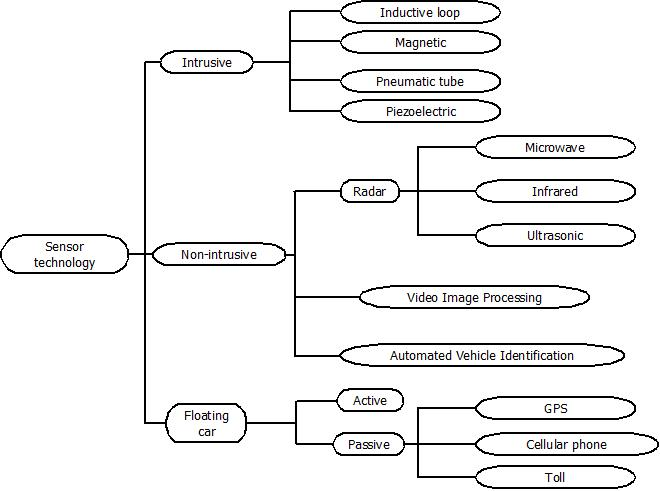
\includegraphics[scale=0.55]{intrusivos.jpeg}  %tipossensores.jpg}
\end{center} 
\caption{Information systems classification, according to the intrusiveness of the technology.} 
\label{tipossensores} 
\end{figure}

Current technologies most frequently used in traffic monitoring include pneumatic tubes, loop detectors, floating vehicles, and automatic recognition systems, among others.


\emph{Manual counts} is the most traditional method. In this case trained observers gather traffic data that cannot be efficiently obtained through automated counts; e.g., vehicle occupancy rate, pedestrians and vehicle classifications. The most common equipments used are tally sheet, mechanical count boards, and electronic count board systems.

\emph{Passive and active infra-red} sensors are based on detecting the presence, speed, and type of vehicles using the infrared energy radiating from the detection area. The main drawbacks are the performance during bad weather, as well as limited lane coverage.

\emph{Microwave radar} can detect moving vehicles and their speed (Doppler radar). It records count data, speed, and simple vehicle classification. Its behaviour is not affected by weather conditions.

\emph{Ultrasonic sensors} devices emit sound waves to detect vehicles by measuring the time for the signal to return to the device. They can be affected by temperature or bad weather. 

\emph{Pneumatic road tubes} are placed across the road lanes to detect the pressure changes produced when a vehicle tyre passes over them. The pulse of air that is created is recorded and processed by a counter located on the side of the road. The main drawback of this technology is that it has limited lane coverage and its efficiency is subject to weather, temperature, and traffic conditions. This system may also not be efficient in measuring low speed flows.
\emph{Piezoelectric sensors} are very similar to pneumatic road tubes, although the principle is to convert mechanical energy into electrical energy. Indeed, mechanical deformation of the piezoelectric material modifies its surface charge density leading to a potential difference that appears between the electrodes. The amplitude and frequency of the signal is directly proportional to the degree of deformation. This system can be used to measure weight and speed.

\emph{Magnetic loops} (inductive, magnetic, or video processing based) may be used temporarily or permanently, the latter being the more usual. 
It is the most conventional technology used to collect traffic data. The loops are embedded in roadways in a square formation that generates a magnetic field. The information is then transmitted to a counting device placed on the side of the road. This has a generally short life expectancy because it can be damaged by heavy vehicles, but is not affected by bad weather conditions. This technology has been widely deployed over the last decades. However, the implementation and maintenance costs can be expensive.

The use of so-called \emph{floating vehicles} consists on a vehicle provided with sensors to collect information while driving on a predefined route.
This active device data collection is one of the most popular among operators of roads, used especially for the collection of travel time and for loop detector calibration.
Depending on the level of automation in the data collection, the cost can vary.

In some areas, such as electronic toll or transit systems, \emph{automatic vehicle identification systems} (AVI) are also widely used. 
These sensors are non-exhaustive data sources to identify tags located in vehicles, such as in payment-systems without stopping. 
The system detects the pass, and the data is sent to the server where it is processed in order to carry out an event (pay toll, opening in the fence, etc).

The main disadvantage of these systems is that they are unable to identify vehicles detected, in order to obtain origin/destination matrixes.
Just the number of vehicles and their type can be calculated, but does not allow to obtain moves flow, nor to determine whether a certain vehicle passes repeatedly.
In addition, its high cost makes it unprofitable covering secondary roads with them, so they are often located on major roads.

Finally, the \emph{automatic recognition} technology has experienced an increase in recent years due to its ability to detect individual vehicles without relying on in-vehicle systems. 
Video image detection is a good example: video cameras record vehicle numbers, type and speed by means of different video techniques, e.g. trip line and tracking. 
Furthermore, they are used for automatic detection of incidents on the road. 
That is the main advantage over previous information systems.
However, system reliability might not be the best, as the system can be sensitive to meteorological conditions.
Moreover, these systems are very costly compared to the previous ones.
Finally, from a privacy point of view, the Spanish Data Protection Agency\footnote{Agencia de Protecci�n de Datos} considers the car license plate as a personal data, so that it would require the user consent.


% ------------------------------------------------------------------------------

\subsubsection{Commercial products}
There are different companies working in the traffic information area using approaches similar to the presented in this work.

\begin{itemize}

\item \textbf{Bit Carrier} \cite{patenteBC} \cite{BitCarrier}: It offers a traffic management system based in BT to count people and commercial routes (pathsolver). Its technology was implanted in highways managed by Abertis for traffic control and monitoring. Actually it has a 150 devices network in Catalonia, so it allows count the traffic times of 200.000 persons each day.
 
\item \textbf{Trafficnow} \cite{Trafficnow}: Another BT system product. A pilot experience has been implanted in Vigo.

 \item \textbf{Traffax Inc} \cite{TraffaxInc}: It is a company that also has used BT for calculating origin-destination and transport time matrixes.

 \item \textbf{Savari Networks} \cite{SavariNetworks}: It offers the commercial product StreetWAVE for traffic monitoring to know in real time the traffic status.


 \item \textbf{TrafficCast} \cite{TrafficCast}: They have developed prediction models in different cities based on different technologies, such as cameras, BT and RFID included in the vehicles.

\end{itemize}

The proposal presented in this work have some common features with the previous approaches, offering similar functionality but with reduced cost.

%===============================================================================

\subsection{Time series forecasting}
\label{subsec:time-series}
Briefly described, a time series is a set of chronologically collected data. Time series forecasting is the task of predicting values of a given series using its own past and present values; the values of any related exogeneous variable can be also used, when available.
Time series forecasting is a major field of research, mainly in the areas of statistics \cite{Gooijer25years} and operational research \cite{Fildes2008}, as time series can be found in fields like Engineering, Biology, Economy, or Social Sciences, among many others.

Time series forecasting is usually tackled trying to find out an underlying model that describes the series behaviour. For this reason, there exist a wide variety of methods to perform forecast using both linear and nonlinear models. The group of linear methods comprises the exponential smoothing methods \cite{Brown1959,Winters1960}, simple exponential smoothing (SES), or State space models \cite{Snyder1985}, among many others. Nevertheless, the most well-known, widely used linear methods are the ARIMA ones \cite{BoxJenk}. ARIMA methods can be summarized as iterative cycles in which: a) the time series is classified as belonging to a pre-established class; b) according to that class, a set of parameters is estimated; and c) the obtained model is verified in other to accept it, or search for another one returning to first step. The models provide by ARIMA integrate in their equations autoregressive (AR) and moving average (MA) components to have into account pass values as well as previous forecasting errors.

Despite their ease of use, linear models have shown no to be accurate for many real applications, being this the main reason why new (but also more complex and difficult to be used) nonlinear methods have been developed. Nonlinear models include regime-switching models, which comprise the wide variety of existing threshold autoregressive (TAR) models \cite{Tong1978}. Clements \cite{Clements2004} exposed main drawbacks of nonlinear methods, mainly the excessively complex models they provide, the lack of robust performance, and, worst of all, the difficulty to use. De Gooijer \cite{Gooijer25years} also concludes that future research on nonlinear models should include, among others, the search for easy to use software.

%\subsection{Soft computing methods for time series forecasting}

Forecasting values for time series has been also faced with soft computing approaches; for instance, the ones by Samanta \cite{Samanta2011} and Zhu \cite{Zhu2011}, who developed methods based on cooperative particle swarm optimization. In \cite{Qiu2011} and \cite{Wang2011} fuzzy time series models are proposed in order to predict new values.Similarly, Yu and Huarng \cite{Yu2010} applied ANNs for training and forecasting in their fuzzy time series model. Models such as support vector regression \cite{Kavaklioglu2011} and fuzzy expert system \cite{Dash1995} were proposed for the electricity demand forecasting, among others.

As can be seen, ANNs have been applied to time series and they are currently recognized as an important tool for forecasting. 

Tang \cite{Tang1991} concluded that ANNs could provide better long-term forecasting; moreover, ANNs can perform better than ARIMA models with short series of input data. Furthermore, contrary to the traditional linear and nonlinear time series models, ANNs are nonlinear data-driven approaches with more flexibility and effectiveness in modeling for forecasting \cite{Zhang1998b}. Jain and Kumar determined in their work \cite{Jain2007} that the ANN models were able to produce more accurate forecasts than traditional models because they do not presuppose any functional form of the model to be developed and they do not depend on the assumptions of linearity.

There exist numerous works of different application areas where ANNs are used to forecast time series. The work by Arizmendi \cite{Arizmendi1993} obtained accurate predictions of the airborne pollen concentrations using ANNs. Zhang and Hu \cite{Zhang1998b} employed ANNs, and Rivas et al. \cite{Rivas04} RBFNs, for forecasting British pound and US dollar exchange rates. Bezerianos et al. \cite{Bezerianos1999} employed RBFNs for the assessment and prediction of the heart rate variability. 

%\subsection{Radial Basic Function Networks}

Specifically inside the ANNs, the use of RBFs as activation functions for them and its application to time series forecasting were firstly considered by Broomhead and Lowe in 1988 \cite{Broomhead88}. Afterwards, new works by Carse and Fogarty \cite{Carse1996}, and Whitehead and Choate \cite{Whitehead96} focused on the prediction of time series.

In later works, Harpham and Dawson \cite{Harpham06} studied the effect of different basis functions on an RBFN for time series prediction. Moreover, Du \cite{Du2008} used time series with an encoding scheme for training RBFNs by GAs. Both the architecture (numbers and selections of nodes and inputs) and the parameters (centers and widths) of the RBFNs were represented in one chromosome and evolved simultaneously by GAs so that the selection of nodes and inputs could be automatically achieved.

Previous works found in literature can also be classified according to the prediction horizon. Thus, forecasting can be divided into short-term, medium-term, and long-term. Generally, forecasting is trended to short-term prediction such as one-step ahead prediction, since longer period prediction (medium-term or long-term) is more difficult, and sometimes may not be reliant because of the error propagation \cite{Chatterjee06}. Thus, neural network models have been traditionally applied in short-term forecasting \cite{Hippert10,Lee09}. For instance, the work by Perez-Godoy \cite{PerezGodoy2010} applied a hybrid evolutionary cooperative-competitive algorithm for the design of RBFNs to the short-term and even medium-term forecasting of the extra-virgin olive oil price.

%\subsubsection{Lags selection}

As mentioned, another problem that emerges working with time series is the correct choice of the lags considered for representing the series. The relationship involving time series historical data defines a $d$-dimensional space where $d$ is the minimum dimension capable of representing such a relationship. Takens' theorem \cite{Takens1980} establishes that if $d$ is sufficiently large is possible to build a state space using the correct time lags and if this space is correctly rebuilt also guarantees that the dynamics of this space is topologically identical to the dynamics of the real systems state space. %Many methods can be found in the literature for the correct definition of the variable $d$, that is, the correct choice of the important time lags of the system dynamics, sometimes called as active dimension of the dynamics generating a time series from the observed series \cite{Tanaka2001}.

In order to tackle the lags selection problem, an evolutionary method that performs a search for the minimum number of dimensions, Time-delay Added Evolutionary Forecasting (TAEF), is presented in \cite{Ferreira2008}. The methodology is inspired in Takens' theorem [***CITA***] and consists of an iterative hybrid model composed of an ANN combined with a genetic algorithm (GA). In \cite{Luko2010} the evolutionary selection of lags is divided into two stages: first, the optimal dimension of the reconstructed phase space is determined by the false nearest neighbors algorithm and then a near-optimal set of time lags is found with a genetic algorithm for a fuzzy inference system.

%In general, these proposals are based on the primary dependences among the variables, do not consider any possible induced dependences, and discard any possible correlation that can exist among the time series parameters, even higher order correlations.
There are some methods that carry out an automatic search of the relevant lags. QIEHI algorithm \cite{Araujo2010a}, for instance, is an evolutionary hybrid intelligent method which is composed of an ANN and a modified evolutionary algorithm to search the minimum dimension to determine the characteristic phase for time series. %The model is built in two stages as in \cite{Ferreira2008}.
Another hybrid methodology composed of a modular morphological ANN with an evolutionary algorithm that searches for the best time lags is described in \cite{Araujo2010b}. %With the same modular morphological neural network, the time lags are obtained by means of a particle swarm optimizer in \cite{Araujo2010c} and by means of a modified GA in \cite{Araujo2011}.
In \cite{garcia2008} a study on the selection not only of the lags but also of the exogenous features with classical feature selection algorithms as pre-processing stage is performed. %The authors show the utility of a feature selection pre-processing stage for time series forecasting with different models.
The lag selection is performed as a post-processing stage in \cite{Maus2011} with a sensitivity computation of the output to each time lag. %The initial stage trains a single-layer, feed-forward ANN based on $d$ time lags, with $d$ chosen large enough to capture the relevant dynamics of the time series. %Another methodology which considers the lag selection as a post-processing stage is
%TDSEP \cite{Sun2006} uses a GA for the optimal selection of time lags for a previously obtained and diagonalized second-order correlation matrices.

As can be observed, the approaches in the literature consider the lags selection as a pre- or post-processing or as a part of the learning process but, instead of together, in hybrid processes with two or three stages. On the contrary, our goal is to address the selection of the lags which represent the series (with any type of correlation) jointly with the design process.

%\subsection{Radial Basic Function Networks}


%%%%%%%%%%%%%%%%%%%%%%%%%%%%%% DATA COLLECTING %%%%%%%%%%%%%%%%%%%%%%%%%%%%%

\section{Data-collecting}
\label{sec:data}

Identifying the MAC address of BT devices passing by the roads has being achieved using Intelify (see Figure \ref{intelify}), a hardware solution with a low power consumption and a high detection range.

\begin{figure}[htpb] 
\begin{center} 
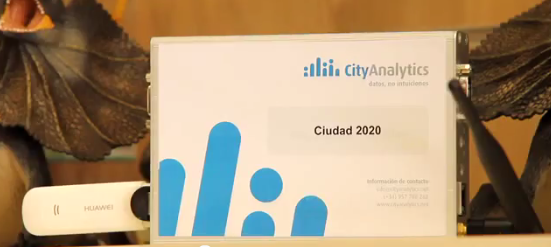
\includegraphics[scale=0.5]{intelifychisme1.png}
\end{center} 
\caption{Intelify device with a connected USB 3G dongle.} 
\label{intelify} 
\end{figure}

Intelify is a small autonomous computer that can be installed in any area to be monitored. It is an autonomous unit, provided by several sensors so that it can discover what is happening in its surroundings (like the flow of people and vehicles). At the same time the environment is been scanned, Intelify is able to send the information to a central server for further processing and interpretation. Table \ref{caracteristicas} shows main features of the device.

\begin{table}[htpb]
\begin{center}
\begin{tabular}{|c|c|}
\hline
Dimensions & 113x163x30mm \\
\hline
     & Power             \\
LEDs & 3G activity       \\
     & Ethernet activity \\
\hline
           & Ethernet  \\
Networking & Wireless  \\
           & Bluetooth \\  
           & 3G        \\
\hline
USB ports & City Analytics Antenna \\
		  & 3G dongle              \\
\hline
Other ports & RS-232 \\
			& VGA    \\
\hline
 	  & 18v - 1200mA          \\
Power & external jack - 5.5mm \\
      & internal jack - 2.1mm \\
\hline
Network     & Ethernet RJ45 \\
connections & 3G USB Modem  \\
\hline
Antennas & City Analytics USB antenna \\
		 & wireless antenna \\
\hline
Microphone & noise sensor \\
\hline
Temperature & main board temperature sensor with extrapolation \\
\hline
Box & 1.5mm aluminum box \\
    & external use possible  \\
\hline
Operating System & Debian 6.0 Squeeze  \\
\hline
\end{tabular}
\end{center}
\caption{Main features of the Intelify device.}
\label{caracteristicas}
\end{table}

This hardware device is based on technology developed by Ciudad 2020 \cite{cityanalytics,Blobject}, and the services it offers are based on a net of Intelify devices. Using such an structure, it has the capacity to discover information about the physical environment and help with decision making to any kind of organization based on people flow and behavior.

Valuable information about tourism, trade and mobility can be gathered through the deployment of autonomous devices around a city. A specific example is the service offered in \cite{numerodepersonas}. It offers information about foot traffic through Cordoba city center.

The cost of this solution is 1000 euros per device, including maintenance of remote computer, communications using a 3G telephony service and storage and data management.

Data accuracy is very representative, compared against other technologies.
In \cite{estudioprecision} it was obtained an a priori error estimation of $8.5\%$ of detections.
%This study \cite{estudioprecision} shows that the average error found in the detection of people is 8.5\%.


??????Descripción de los datos recopilados


%%%%%%%%%%%%%%%%%%%%%%%%%%%% EXPERIMENTS AND RESULTS %%%%%%%%%%%%%%%%%%%%%%%%%%%

\section{Experiments and results}
\label{sec:experiments}

????? TODO ESTO HAY QUE CAMBIARLO PARA LOS DATOS REALES CON LSO QUE AL FINAL HEMOS TRABAJADO

In this section the analysis of collected data during the monitoring period (November 8 to December 9) to obtain statistics and so study the use of vehicles is carried out.

 % Concretamente, en las siguientes subsecciones, reportaremos información acerca del número total de vehículos detectados por cada nodo, en días laborables o festivos, sobre la densidad del tráfico por rango horario, acerca de los desplazamientos individuales, y de la velocidad media en un tramo delimitado por dos nodos consecutivos.
Specifically, the following subsections report information about the total number of vehicles detected by each node, on weekdays or holidays, information on traffic density by time range on individual movements, and the average speed on a section delimited by two consecutive nodes.

 % Por último, puesto que el día 14 de noviembre de 2012 se celebró la huelga general, estudiaremos cómo afectó la huelga al tráfico en el área metropolitana de Granada, comparando los totales de detección de dispositivos entre el día de la huelga (14 de noviembre), y el miércoles siguiente (21 de noviembre).
Finally, since November 14 2012 a general strike was held, we will study how the strike affected traffic in the metropolitan area of Granada (Spain), by comparing total number of devices detected that day (November 14), and the following day (November 15).

%===============================================================================

\subsection{Total number of vehicles detected (weekdays and holidays)}
 % VehiculosTotales.txt tiene los vehículos totales detectados en cada nodo.

% La primera parte del análisis ha consistido en calcular el número de dispositivos detectados por cada uno de los nodos instalados.
The first analysis consisted in calculating the number of devices detected by each node.

 \begin{table}
 \begin{center}
 \begin{tabular}{|c|c|}
 \hline
Node Id.  &  N. of devices detected  \\
 \hline
    1     &    31408  \\
 \hline
    2     &    45032  \\
 \hline
    3     &    33165  \\
 \hline
    4     &    358494  \\
 \hline
    5     &    297874  \\
 \hline
    6     &    7872  \\
 \hline
 \end{tabular}
 \end{center}
 \caption{Number of BT devices detected by each node.
 \label{VehiculosTotales}}
 \end{table}

 % En total se han detectado 773845 dispositivos BT al paso por los seis nodos. 
 % Como se observa en la Tabla \ref{VehiculosTotales}, los dos nodos situados en la autovía de Sierra Nevada (A44, Circunvalación de Granada, nodos 4 y 5) son los que más datos han recogido, mientras que el situado en una calle secundaria (nodo 6) ha sido el que menos dispositivos ha recogido.

In total, 773,845 BT devices have been detected by the six nodes.
As shown in Table \ref{VehiculosTotales}, nodes located in the Sierra Nevada Highway (A44, nodes 4 and 5) have collected a higher number of data, while the node located in a side street (node 6) has detected the smallest number of devices.

%===============================================================================

\subsection{Total vehicles detected on non-working days}
 % VehiculosFestivos.txt tiene los vehículos detectados en día festivo en cada nodo.

 % A continuación, y para comparar la intensidad circulatoria entre días laborables y no laborables, se ha calculado el número de pasos en días festivos y no laborables.
To compare the traffic intensity between working and non-working days, the number of pass on holidays and non-working days have been obtained.

 \begin{table}
 \begin{center}
 \begin{tabular}{|c|c|}
 \hline
Node Id.  &  N. of devices detected  \\
 \hline
    1     &    2149  \\
 \hline
    2     &    2804  \\
 \hline
    3     &    2832  \\
 \hline
    4     &    32182  \\
 \hline
    5     &    24166  \\
 \hline
    6     &    1269  \\
 \hline
 \end{tabular}
 \end{center}
 \caption{Total number of BT devices detected by each node (only on non-working days).
 \label{VehiculosFestivos}}
 \end{table}

 % La Tabla \ref{VehiculosFestivos} muestra un descenso en el número de dispositivos detectados por todos los nodos en días no laborables, frente al número de detecciones en días laborables. 
 % Aún así, los nodos situados en la autovía de Sierra Nevada siguen recogiendo muchos más datos que el resto, debido al tráfico denso que soporta esta vía en días no laborables.

Table \ref{VehiculosFestivos} shows how the number of detected devices lowers by all nodes on non-working days, compared to the number of detections on weekdays.
Nodes located in the Sierra Nevada Highway still collected much more data than the remainder, due to the traffic this road supports on holidays.

%===============================================================================

\subsection{Traffic density on the road by time range}
 % VehiculosDiferentesPorHoras.txt contiene para cada uno de los nodos, los dispositivos diferentes detectados en cada rango horario (final de la línea)

 % La densidad circulatoria por horas podemos calcularla a partir del total de dispositivos diferentes detectados en cada rango horario.
Traffic density can be calculated taking into account the total number of detected devices by time range.

 \begin{figure}[htb]
 \begin{center}
 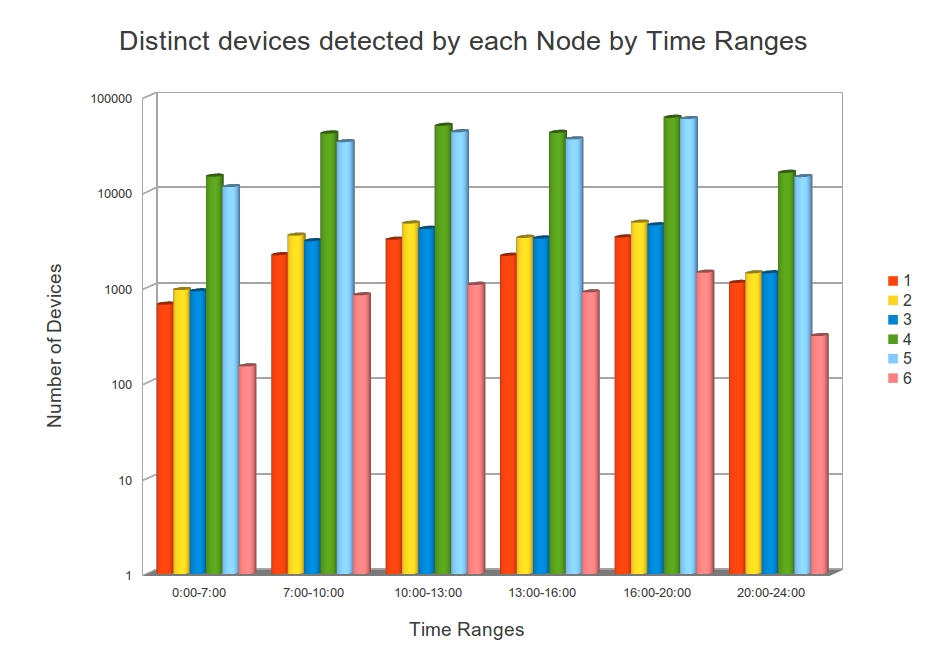
\includegraphics[scale=0.4]{VehiculosDiferentesPorHoras.jpg}
 \caption{For each node, the total number of different detected devices by time range is shown. Figure is shown in logarithmic scale.
 % Para cada uno de los nodos se muestra el total de dispositivos diferentes detectados en cada rango horario. Para cada rango de horas se muestra el total detectado en cada uno de los seis nodos
 \label{VehiculosDiferentesPorHoras}}
 \end{center}
 \end{figure}
 % Gráfica (histograma) de la densidad de la vía por horas: desde las 00-7h, de 7-10h, de 10-13h, de 13-16h, de 16-20h, y de 20-24h.
 
 % La Figura \ref{VehiculosDiferentesPorHoras} muestra mayor densidad, en todos los nodos, a las horas punta de entrada o salida del trabajo y colegios.
Figure \ref{VehiculosDiferentesPorHoras} shows higher density on all nodes, at peak times or out of work and school.

%===============================================================================

\subsection{Total detections by time range}
 % VehiculosPorHoras.txt indica para cada nodo, el número de dispositivos detectados en el rango horario, sin diferenciar si el dispositivo es siempre el mismo o no. 

 % Adicionalmente podemos calcular para cada nodo, el número de dispositivos detectados en cada rango de horas, sin diferenciar si el dispositivo es siempre el mismo o no. Así pues, se incluirán pasos repetidos del mismo vehículo.
Additionally we can calculate for each node, the number of detected devices by time range, without differentiating whether the device is the same or not (repeated passes). Thus, repeated passes of the same vehicle are counted.

 \begin{figure}[htb]
 \begin{center}
 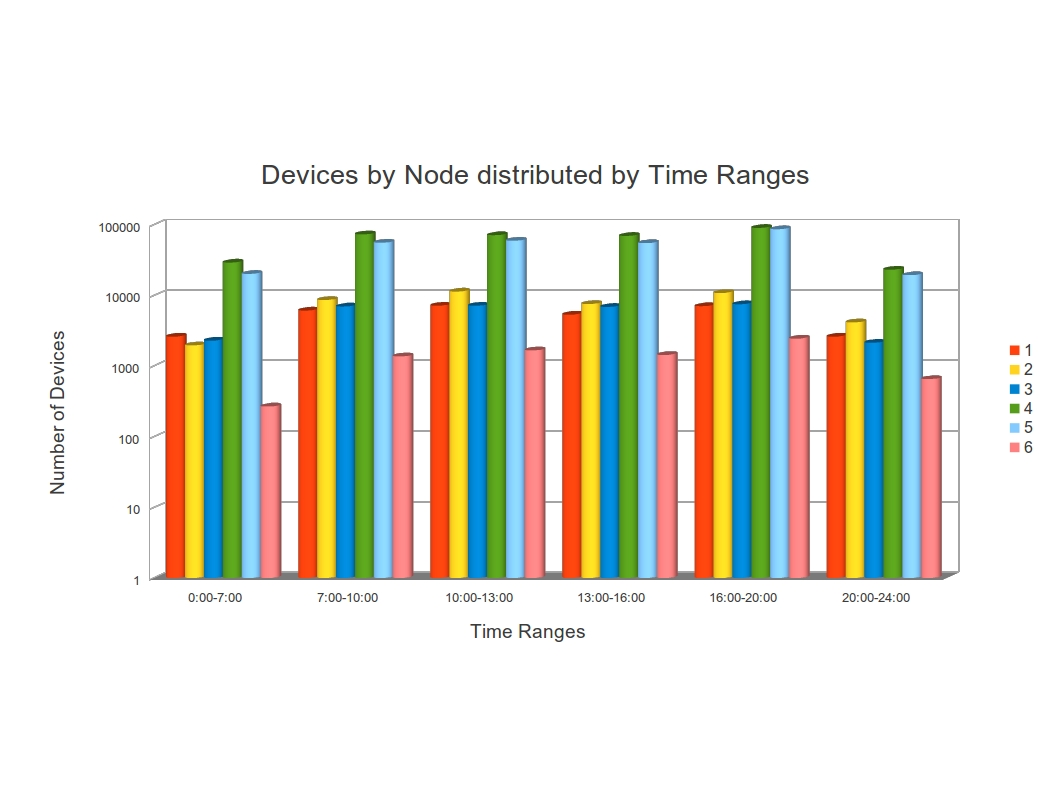
\includegraphics[scale=0.4]{VehiculosPorHoras.jpg}
 \caption{For each of the six nodes, the total number of detected devices by time range is shown. Figure is shown in logarithmic scale.
 % Para cada uno de los nodos se muestra el total de dispositivos detectados en cada rango horario. Para cada rango de horas se muestra el total detectado en cada uno de los seis nodos
 \label{VehiculosPorHoras}}
 \end{center}
 \end{figure}
 
 % Al igual que en el caso anterior, observamos una mayor densidad circulatoria en todos los nodos, a las horas punta de entrada o salida del trabajo y colegios (ver la Figura \ref{VehiculosPorHoras}).
As in the previous case, a greater traffic density can be observed on all nodes, at peak times or out of work and school. (see Figure \ref{VehiculosPorHoras}).

%===============================================================================

\subsection{Number of individual vehicles detections}
 % Intervalos.txt contine el número de vehículos detectados entre 0 y 5 veces, entre 5 y 10 veces y así sucesivamente hasta más de 25 veces detallado en cada nodo.

 % A continuación podemos sacar partido de la capacidad del sistema propuesto para individualizar los dispositivos BT, pudiendo detectar si esos mismos vehículos repiten paso por diferentes nodos.
We can take advantage of the proposed system's ability to identify BT devices. Thus, it can be detected whether vehicles pass by different nodes.

 \begin{figure}[htb]
 \begin{center}
 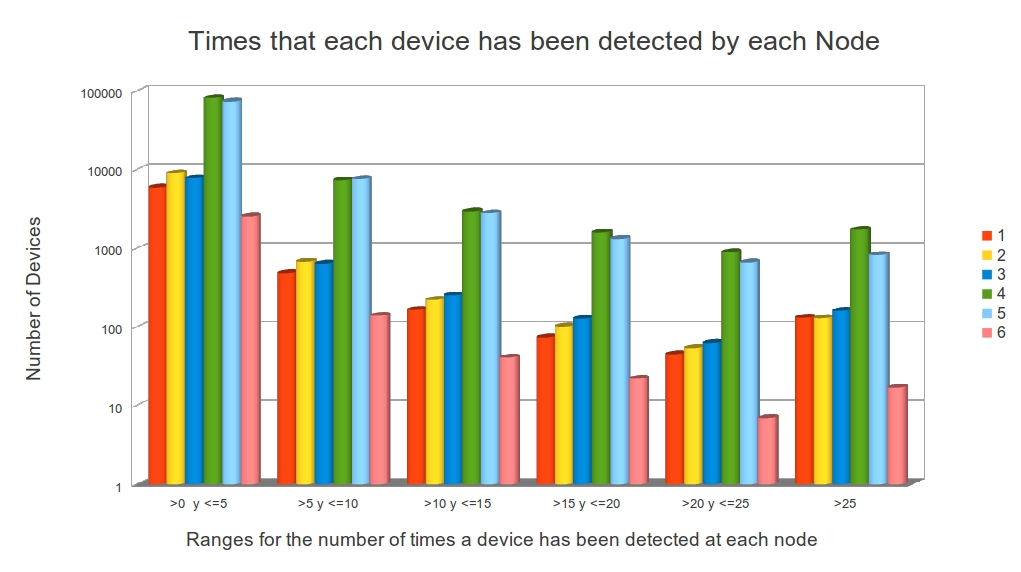
\includegraphics[scale=0.4]{Intervalos.jpg}
 \caption{For each of the six nodes, the total number of detected devices N times (repeated occurrences of the same device) are shown. Figure is shown in logarithmic scale.
 % Para cada uno de los nodos se muestra el total de dispositivos detectados cierto número de veces (repetidas apariciones del mismo dispositivo)
 \label{Intervalos}}
 \end{center}
 \end{figure} 
 % Histograma que muestre cuántos coches se detectan entre una y 5 veces, entre 6 y 10, entre 10 y 20, y más de 20 veces.

 % En la Figura \ref{Intervalos} podemos ver que hay una gran cantidad de vehículos que repiten su paso por ciertos nodos (principalmente los situados en la A44) hasta 10 veces. 
 % Incluso se puede ver que en los nodos 4 y 5 hay alrededor de 1000 vehículos que repiten su paso más de 25 veces. En el resto de nodos, más de 25 repeticiones del mismo dispositivo se han detectado alrededor de 120 veces solamente.

Figure \ref{Intervalos} shows a large number of vehicles that pass repeated times (up to 10 times) by some of the nodes (mainly those located in the A44).
Even it can be seen that nodes 4 and 5 detect about 1,000 vehicles passing more than 25 times repeated. 
On the other nodes, over 25 repetitions of the same device have been detected only around 120 times.

%===============================================================================

\subsection{Complexity of displacement}
 % NodosPorDondePasan.txt contiene el número de vehículos que han pasado por 2 nodos, por 3 nodos y así hasta por los 6 nodos y el número medio de veces que han pasado 2, 3, 4, 5 o 6 veces por cada nodo.

 % En el estudio de la complejidad de los desplazamientos se han calculado el número de vehículos que han pasado por 2 nodos, por 3 nodos y hasta 6 nodos. En la Tabla \ref{tNodosPorDondePasan} se muestra además el número medio de veces que han pasado un vehículo por 2, 3, 4, 5 o 6 nodos.
To study the complexity of displacements, the number of vehicles that have passed through two nodes, 3 nodes and up to 6 nodes  were calculated. 
Table 4 also shows the average number of times that vehicles have passed through 2, 3, 4, 5 or 6 nodes.

 \begin{table}
 \begin{center}
 \begin{tabular}{|c|c|c|c|}
 \hline
 No. of nodes & 	No. of devices & 	Total number of passes & 	Mean $\pm$ std. dev.  \\
 \hline
1 & 	72989 & 	 165033 & 	$2.26 \pm 31.16$  \\
 \hline
2 & 	53947 & 	 425667 & 	$7.89 \pm 11.48$  \\
 \hline
3 & 	8125 & 	 131570 & 	$16.19 \pm 24.71$  \\
 \hline
4 & 	1359 & 	 39241 & 	$28.88 \pm 140.82$  \\
 \hline
5 & 	254 & 	 8603 & 	$33.87 \pm 59.51$  \\
 \hline
6 & 	61 & 	 3731 & 	$61.16 \pm 94.78$  \\
 \hline
 \end{tabular}
 \end{center}
 \caption{Total number of vehicles that have passed through two nodes, 3 nodes and up to 6 nodes, and average number of times that vehicles have passed through 2, 3, 4, 5 or 6 nodes. In some cases the deviations are high because some devices have a very high number of occurrences for some nodes.
 % Número de vehículos que han pasado por 2 nodos, por 3 nodos y hasta 6 nodos, y el número medio de veces que han pasado los vehículos por 2, 3, 4, 5 o 6 nodos. En algunos casos las desviaciones son altas debido a que algunos dispositivos tienen un número muy alto de apariciones por algunos de los nodos
 \label{tNodosPorDondePasan}}
 \end{table}

 % La información anterior se complementa visualmente con la Figura \ref{fNodosPorDondePasan}, en la que se muestra (en escala logarítmica) cuántos coches pasan sólo por un nodo, por dos nodos, por tres nodos, etc.
The above information is complemented with Figure \ref{fNodosPorDondePasan}, that shows how many cars pass by only one node, two nodes, three nodes, etc.

 \begin{figure}[htb]
 \begin{center}
 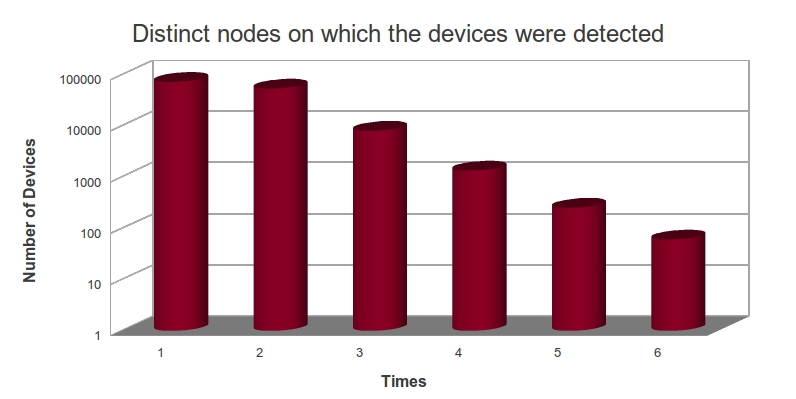
\includegraphics[scale=0.4]{NodosPorDondePasan.jpg}
 \caption{Figure shows how many cars pass by only one node, two nodes, three nodes, etc. Figure is shown in logarithmic scale.
 % La figura muestra cuántos coches pasan sólo por un nodo, por dos nodos, por tres nodos, etc. Para mejorar la visualización se ha utilizado escala logarítmica
 \label{fNodosPorDondePasan}}
 \end{center}
 \end{figure}
 % Histograma que muestre cuántos coches pasan sólo por un nodo, por dos nodos, por tres nodos, etc.

 % Como se esperaba, gran parte de los dispositivos BT pasan pocas veces por casi todos los nodos, mientras que la mayoría pasa sólo por uno o dos de ellos (sus desplazamientos se centran en una parte de la zona pequeña monitorizada).
As expected, most of the BT devices rarely passed by all nodes, while most of devices pass only by one or two of nodes (their displacements are focused on a small part of the monitored area).

%===============================================================================

\subsection{Effect of Nov-14 strike on zone traffic}
 % Tabla en la que mostremos cómo afectó el día 14-N con la huelga.

 % Justo en mitad del periodo de monitorización, en España se celebró un día de huelga general (14 de noviembre de 2012), lo que ha quedado reflejado en la cantidad de coches detectados en los nodos.

 % Se ha analizado el efecto de la huelga general en el tráfico de la zona monitorizada, mostrando en la Tabla \ref{huelga} el número de pasos detectados el día 14 de noviembre y justo el día siguiente.

Right in the middle of the monitoring period in Spain was held a day of general strike (November 14, 2012), which has been reflected in the number of detected devices (cars) on the nodes.

The effect of the general strike in the traffic of the monitored area has been analyzed and shown in Table \ref{huelga} as the number of detected devices on November 14 and the very next day.

 \begin{table}
 \begin{center}
 \begin{tabular}{|c|c|c|}
 \hline
 Node  &  Total number of passes (nov-14) & Total number of passes (nov-15) \\
 \hline
 2	& 1841  & 2722  \\
 \hline
 3	& 891   & 1169 \\
 \hline
 4	& 10807	& 16942 \\
 \hline
 5	& 831  	& 4017\\
 \hline
 6	& 946   & 1419 \\
 \hline
 \end{tabular}
 \end{center}
 \caption{Comparison of the number of passes for each node between the general strike day (November 14) and the very next day. Node 1 results are not reported because the hardware device suffered a power supply problem for a couple of days at that time.
 % Comparación del número de pasos por cada nodo entre el día de la huelga general (14 de noviembre) y el día siguiente. No aparece recogido el nodo 1 debido a que el dispositivo hardware sufrió un problema de alimentación durante un par de días en esas fechas
 \label{huelga}}
 \end{table}

 % En la Tabla \ref{huelga} se aprecia un número de vehículos detectados menor el día de la huelga respecto al día siguiente (laborable en el que la actividad debió ser normal en la zona).
Table 8 shows a lowest number of detected vehicles the day of the strike that on the following day (working day in which the activity should be normal in the area).

%===============================================================================

\subsection{Analysis of vehicles speed between two consecutive nodes}
 % tabla de la velocidad media de los vehículos en el tramo (en laborables y en fin de semana).
 % El "Granada 5" está en el km 123,250 ; el "Granada 4" está en el km 119,550 ; hay 3700 metros entre ambos. 

 % Por último, a partir de los dos nodos consecutivos localizados en la autovía A44, podemos calcular velocidades medias en el tramo delimitado por los nodos 4 (situado en el km 119,550) y 5 (situado en el km 123,250) de un total de 3700 metros. 
 % En realidad podemos calcular la velocidad media en el tramo a nivel global, no la velocidad a la que ha ido cada vehículo en cada instante dentro del tramo.

Finally, taking two consecutive nodes, located on the A44 highway, average speeds in the section bounded by nodes 4 (located at km 119.550) and 5 (located at km 123.250) can be calculated.
This highway section where the study takes place is of 3700 meters long.
Actually, we can calculate the average speed in the global section, not the speed at which each vehicle has at each instant within the section.

 \begin{table}
 \begin{center}
 \begin{tabular}{|c|c|}
 \hline
Speed range (km/h) &  No. of passes  \\
 \hline
v$\leq$60.0	& 1495  \\
 \hline
60.0$\leq$v$\leq$70.0 & 2585  \\
 \hline
70.0$\leq$v$\leq$80.0 & 7421  \\
 \hline
80.0$\leq$v$\leq$90.0 & 16339  \\
 \hline
90.0$\leq$v$\leq$100.0 & 20144  \\
 \hline
100.0$\leq$v$\leq$120.0 & 14384  \\
 \hline
120.0$\leq$v$\leq$140.0 & 5434  \\
 \hline
v$\geq$140.0 & 1326  \\
 \hline
 \end{tabular}
 \end{center}
 \caption{Average speeds (globally) in the section bounded by nodes 4 and 5.
  % Velocidades medias (a nivel global) en el tramo delimitado por los nodos 4 y 5
 \label{velocidad}}
 \end{table}


 % En dicho tramo, la velocidad está limitada a 100 km/h. Sin embargo, y aunque la gran mayoría respetan el límite, vemos que una gran cantidad de coches superan dicha limitación.
In that section, the speed is limited to 100 km/h. However, although most of the vehicles respect this limit, a lot of cars exceed this limitation.

%===============================================================================

\subsection{Flow traffic prediction by means of time-series forecasting}
As far as data is chronologically collected, methods coming from the area of time-series forecasting can be used in order to predict future behaviour of traffic flow.

From the big variety of existing mtethods, 6 different ones have been selected in order to compare the validity of their predictions. The methods being used are the followings: ARIMA, Croston, Theta, Spline,L-Co-R, and as control algorithm, the mean value. Methods  ARIMA, Croston, Theta, Spline and Mean have been executed using the R software, by means of the Forecast package (cita). In the other hand, L-Co-R is a co-evolutionary algorithm of our own, based on radial basis function neural networks. In order to compare the methods, a statistical study is included allowing us to draw some conclusions.

The experimentation has been carried out using the data collected for five nodes over 62 days. The first 55 days have been used to train the methods, and obtain their associated models, and the remaining 7 days have been used to test their generalization capabilities. The prediction has been for an horizon of 1, so that known data until day $n$ have been used to forecast day $n+1$. 

For each method and each node, a set of measures have been computed in order to determine the accuracy of the prediction. As most textbooks recommend, one of the chosen measures is  the Mean Absolute Percentage Error (MAPE) \cite{Bowerman2004}, which was used in the first M-competition \cite{Makridakis1982}. Median Absolute Percentage Error (MdAPE) \cite{Armstrong,Fildes1992} is also used, as a normalized version of the previous one. More recently, the description of many others measures can be found in  \cite{Gooijer25years} and \cite{Hyndman2006}. Among all of them, in this work we use the followings:

\begin{itemize}
  \item Mean Absolute Error (MAE):
        \begin{equation}\label{eq:MAE}
            MAE = mean(\mid e_t\mid)
        \end{equation}

  \item Mean Absolute Percentage Error (MAPE):
        \begin{equation}\label{eq:MAPE}
            MAPE = mean(\mid p_t\mid)
        \end{equation}

        \bigskip
  \item Median Absolute Percentage Error (MdAPE):
        \begin{equation}\label{eq:MDAPE}
            MdAPE = median(\mid p_t\mid)
        \end{equation}

  \item Mean Absolute Scaled Error (MASE):
        \begin{equation}\label{eq:MASE}
            MASE = mean(\mid q_t\mid)
        \end{equation}

  \item Mean Squared Error (MSE):
        \begin{equation}\label{eq:MSE}
            MSE = \frac{1}{n}\sum_{i=1}^n {e_t}^2
        \end{equation}

%  \item Root Mean Squared Error (RMSE):
%        \begin{equation}\label{eq:RMSE}
%            RMSE = \sqrt{\frac{1}{n}\sum_{i=1}^n {e_t}^2}
%        \end{equation}


where $Y_t$ is the observation at time $t = {1,...,n}$; $F_t$ is the forecast of $Y_t$; $e_t$ is the forecast error (i.e. $e_t= Y_t - F_t$); $p_t = 100e_t/Y_t$ is the percentage error, and
         $q_t = \displaystyle\frac{e_t}{\displaystyle\frac{1}{n-1} \sum_{i=2}^n \mid Y_i - Y_{i-1} \mid }$
\end{itemize}

Given the stochastic nature of evolutionary algorithms, and in order to remove biases due to random generator, L-Co-R has been running 30 times per node. Thus, the error attached to this algorithm correspond to the average error values of these 30 executions.

Table \ref{tb:ts-results} show the different error values for every method and node. Boldfaces highlight  the lowest (best) values per algorithm, node and measure. As table shows, best algorithms tends to be L-Co-R and ARIMA, since L-Co-R obtains the lowest results for measures MAE, MAPE, MdAPE and MASE (except for node 2), but there is not a clear winner in MSE and SMAPE.


\begin{table} \footnotesize
 \begin{center}
 \begin{tabular}{|l|c|c|c|c|c|c|c|}


\hline 
 \multicolumn{7}{|c|}{Node 1} \\ 
 \hline 
 & \emph{MAE} & \emph{MAPE} & \emph{MASE} & \emph{MdAPE} & \emph{MSE} & \emph{SMAPE} \\ 
\hline

\emph{ARIMA } & $514,83$ & $40,42$ & $1,14$ & $30,76$ & $424860,5$ & $36,83$ \\ 
\emph{CROSTON } & $509,91$ & $39,28$ & $1,13$ & $33,8$ & $387403,9$ & $36,46$ \\ 
\emph{THETA } & $528,59$ & $41,16$ & $1,17$ & $32,78$ & $443898,5$ & $37,87$ \\ 
\emph{SPLINE } & $550,02$ & $43,87$ & $1,21$ & $30,1$ & $488504,9$ & $39,04$ \\ 
\emph{MEAN } & $456,95$ & $38,57$ & $1,01$ & $26,11$ & $318623,5$ & $32,48$ \\ 
\emph{L-Co-R} & $\textbf{372,77}$ & $\textbf{23,66}$ & $\textbf{0,81}$ & $\textbf{18,46}$ & $\textbf{231731,8}$ & $\textbf{28,87}$ \\ 
\hline 
 \multicolumn{7}{|c|}{Node 2} \\ 
 \hline 
 & \emph{MAE} & \emph{MAPE} & \emph{MASE} & \emph{MdAPE} & \emph{MSE} & \emph{SMAPE} \\ 
\hline

\emph{ARIMA } & $433,52$ & $26,64$ & $\textbf{1,03}$ & $22,38$ & $\textbf{310105,3}$ & $25,15$ \\ 
\emph{CROSTON } & $532,87$ & $27,98$ & $1,26$ & $27,89$ & $398979,9$ & $30,5$ \\ 
\emph{THETA } & $435,58$ & $26,77$ & $1,03$ & $22,55$ & $312496,1$ & $25,28$ \\ 
\emph{SPLINE } & $535,86$ & $34,53$ & $1,27$ & $24,7$ & $447557,4$ & $31,17$ \\ 
\emph{MEAN } & $489,57$ & $24,44$ & $1,16$ & $28,64$ & $361070,5$ & $27,52$ \\ 
\emph{L-Co-R} & $\textbf{429,78}$ & $\textbf{11,41}$ & $1,04$ & $\textbf{11,98}$ & $311561,7$ & $\textbf{23,5}$ \\ 
\hline 
 \multicolumn{7}{|c|}{Node 3} \\ 
 \hline 
 & \emph{MAE} & \emph{MAPE} & \emph{MASE} & \emph{MdAPE} & \emph{MSE} & \emph{SMAPE} \\ 
\hline

\emph{ARIMA } & $373,17$ & $35,11$ & $1,32$ & $27,54$ & $\textbf{150293,6}$ & $\textbf{33,45}$ \\ 
\emph{CROSTON } & $377,42$ & $37,03$ & $1,34$ & $27,89$ & $160970,9$ & $33,78$ \\ 
\emph{THETA } & $394,95$ & $38,11$ & $1,4$ & $29,41$ & $175710,7$ & $35,34$ \\ 
\emph{SPLINE } & $384,68$ & $38,86$ & $1,36$ & $29,36$ & $184807,2$ & $34,36$ \\ 
\emph{MEAN } & $373,18$ & $35,11$ & $1,32$ & $27,53$ & $150307,8$ & $33,45$ \\ 
\emph{L-Co-R} & $\textbf{363,3}$ & $\textbf{10,56}$ & $\textbf{0,84}$ & $\textbf{17,01}$ & $182469,9$ & $35,32$ \\ 
\hline 
 \multicolumn{7}{|c|}{Node 4} \\ 
 \hline 
 & \emph{MAE} & \emph{MAPE} & \emph{MASE} & \emph{MdAPE} & \emph{MSE} & \emph{SMAPE} \\ 
\hline

\emph{ARIMA } & $3168,36$ & $40,62$ & $1,04$ & $18,99$ & $21792093$ & $37,44$ \\ 
\emph{CROSTON } & $3789,4$ & $56,83$ & $1,25$ & $54,33$ & $25037291$ & $49,12$ \\ 
\emph{THETA } & $3085,3$ & $38,14$ & $1,01$ & $25,42$ & $21510757$ & $37,48$ \\ 
\emph{SPLINE } & $3758,06$ & $39,45$ & $1,24$ & $43,53$ & $28745309$ & $48,79$ \\ 
\emph{MEAN } & $4545,17$ & $92,73$ & $1,5$ & $40,07$ & $26612429$ & $55,57$ \\ 
\emph{L-Co-R} & $\textbf{540,59}$ & $\textbf{6,26}$ & $\textbf{0,07}$ & $\textbf{4,14}$ & $\textbf{1120317,2}$ & $\textbf{8,17}$ \\ 
\hline 
 \multicolumn{7}{|c|}{Node 5} \\ 
 \hline 
 & \emph{MAE} & \emph{MAPE} & \emph{MASE} & \emph{MdAPE} & \emph{MSE} & \emph{SMAPE} \\ 
\hline

\emph{ARIMA } & $5012,95$ & $43,8$ & $1,13$ & $20,19$ & $\textbf{29974781}$ & $\textbf{33,85}$ \\ 
\emph{CROSTON } & $5583,14$ & $46,32$ & $1,26$ & $26,12$ & $35082013$ & $37,51$ \\ 
\emph{THETA } & $5779,37$ & $45,78$ & $1,3$ & $28,25$ & $35859271$ & $38,94$ \\ 
\emph{SPLINE } & $5878,35$ & $46,26$ & $1,32$ & $28,69$ & $37288518$ & $39,64$ \\ 
\emph{MEAN } & $5013,48$ & $43,81$ & $1,13$ & $20,19$ & $29980578$ & $33,85$ \\ 
\emph{L-Co-R} & $\textbf{4978,08}$ & $\textbf{24,59}$ & $\textbf{0,87}$ & $\textbf{9,37}$ & $35875329$ & $35,8$ \\ 


\hline

 \end{tabular}
 \end{center}
 \caption{Values for the six error measures (MAE, MAPE, MASE, MdAPE, MSE, and SMAPE) yielded for any of the six methods (ARIMA, Croston, Theta, Spline, Mean and L-Co-R) when forecasting time series of nodes 1 to 5. Boldfaces stress best (lowest) values.
 \label{tb:ts-results}}
 \end{table}

The results yielded by every method have been compared using two non-parametric test: the Friedman test and the Iman-Davenport test. Using this two test, we are able to determine whether there exist significant differences between the methods or not, and we can establish a ranking of methods according to their ability to perform forecast. These test have been carried out using ??? SOFTRWAE DE SALVA. Both, Friedman and Iman-Davenport tests, reveal that results can be considered significantly differents when the computed \emph{P-value} is less than $0.05$. Table \ref{tb:friedman-iman-tests} shows that any of the \emph{P-value} computed by the tests are under $0.05$, and this occurs in any of the six error measures being considered.



\begin{table} \footnotesize
 \begin{center}
 \begin{tabular}{|l|c|c|}
\hline
\emph{Error} & \emph{Friedman P-value} & \emph{Iman-Davenport P-value} \\
\hline
\emph{MAE} & $0.0052$ & $0.0003$ \\
\emph{MAPE} & $0.0080$ & $0.0008$ \\
\emph{MASE} & $0.0141$ & $0.0030$ \\
\emph{MdAPE} & $0.0063$ & $0.0005$ \\
\emph{MSE} & $0.0213$ & $0.0066$ \\
\emph{SMAPE} & $0.0440$ & $0.0233$ \\
\hline

 \end{tabular}
 \end{center}
 \caption{\emph{P-value} yielded by Friedman and Iman-Davenport non-parametrics tests for every error measure. A \emph{P-value} lower than $0.05$ (all of them in this case) indicates that there exist significant differences between the errors computed for every method.
 \label{tb:friedman-iman-tests}}
 \end{table}

Futhermore, Friedman test results also provide a mechanism to establish a ranking between the methods, determining which one can be considered the best. Once the method has been found out, it can be compared against the rest methods using the Holm's procedure (�???CITA). This method computes the probability that two methods can be considered to have a similar behaviour, being this the null hypothesis. The null hypothesis is rejected when this probability is lower than $0.05$, so that methods can be considered to be significantly differents. For instance, table \ref{tb:holm-mae} shows the probabilities computed by the Holm's procedure for error MAE; L-Co-R does not appear in the table since it results to be the best method with respect to this error, and it is taken as control algorithm. According to the values shown, there are not signficant differences between L-Co-R and ARIMA, but there exist between L-Co-R and the rest of methods.


\begin{table}[!htp]\footnotesize
\begin{center}
\begin{tabular}{|cccccc|}
\hline
\emph{Error}&\emph{Control Method}&\emph{Ranking}&
\emph{Method}&$p$& \emph{Null Hypothesis}\\
\hline
&&1&ARIMA&0.176&Accepted\\
&&2&MEAN&0.028& \textbf{Rejected}\\
MAE&L-Co-R&3&THETA&0.007& \textbf{Rejected}\\
&&4&CROSTON&0.007& \textbf{Rejected}\\
&&5&SPLINE&2.003E-4& \textbf{Rejected}\\
\hline
&&1&ARIMA&0.090& Accepted\\
&&2&MEAN&0.0.063& Accepted \\
MAPE&L-Co-R&3&THETA&0.011& \textbf{Rejected}\\
&&4&CROSTON&0.002& \textbf{Rejected}\\
&&5&SPLINE&3.857E-4& \textbf{Rejected}\\
\hline
&&1&ARIMA&0.398& Accepted\\
&&2&MEAN&0.063& Accepted \\
MASE&L-Co-R&3&THETA&0.028& \textbf{Rejected}\\
&&4&CROSTON&0.018& \textbf{Rejected}\\
&&5&SPLINE&7.232E-4& \textbf{Rejected}\\
\hline
&&1&ARIMA&0.176&Accepted\\
&&2&MEAN&0.042& \textbf{Rejected}\\
MdAPE&L-Co-R&3&THETA&0.004& \textbf{Rejected}\\
&&4&SPLINE&0.002& \textbf{Rejected}\\
&&5&CROSTON&7.232E-4& \textbf{Rejected}\\
\hline
&&1&L-Co-R&0.500&Accepted\\
&&2&MEAN&0.398& Accepted \\
MSE&ARIMA&3&CROSTON&0.176& Accepted \\
&&4&THETA&0.176& Accepted \\
&&5&SPLINE&7.232E-4& \textbf{Rejected}\\
\hline
&&1&L-Co-R&0.866& Accepted\\
&&2&MEAN&0.310& Accepted \\
SMAPE&ARIMA&3&CROSTON&0.091 & Accepted \\
&&4&THETA&0.043& \textbf{Rejected}\\
&&5&SPLINE&0.006& \textbf{Rejected}\\
\hline
\end{tabular}
\end{center}
\caption{Results of the Holm's procedure for every error. Values of $p$ under or equals to $0.05$ lead to reject the null hypothesis, i.e., the errors provided by the control algorithm and the corresponding compared algorithm can be considered significantly differents.
\label{tb:holm-all}}

\end{table}

Holm's procedure has been applied to any of the six error measure being considered. Table \ref{tb:holm-all} summarizes the rankings of methods, as well as the existence or absence of significant differences. Thus, this statistic study shows that L-Co-R is the best algorithm in four of six error measures; nevertheless, it can not be said to be better than ARIMA in any case but, for most measures, it overcomes the rest of methods.





%%%%%%%%%%%%%%%%%%%%%%%%% CONCLUSIONS AND FUTURE WORK %%%%%%%%%%%%%%%%%%%%%%%%%%

\section{Conclusions and Future Work}
\label{sec:conclusions}


%% The Appendices part is started with the command \appendix;
%% appendix sections are then done as normal sections
%% \appendix

%% \section{}
%% \label{}

%% References
%%
%% Following citation commands can be used in the body text:
%%
%%  \citet{key}  ==>>  Jones et al. (1990)
%%  \citep{key}  ==>>  (Jones et al., 1990)
%%
%% Multiple citations as normal:
%% \citep{key1,key2}         ==>> (Jones et al., 1990; Smith, 1989)
%%                            or  (Jones et al., 1990, 1991)
%%                            or  (Jones et al., 1990a,b)
%% \cite{key} is the equivalent of \citet{key} in author-year mode
%%
%% Full author lists may be forced with \citet* or \citep*, e.g.
%%   \citep*{key}            ==>> (Jones, Baker, and Williams, 1990)
%%
%% Optional notes as:
%%   \citep[chap. 2]{key}    ==>> (Jones et al., 1990, chap. 2)
%%   \citep[e.g.,][]{key}    ==>> (e.g., Jones et al., 1990)
%%   \citep[see][pg. 34]{key}==>> (see Jones et al., 1990, pg. 34)
%%  (Note: in standard LaTeX, only one note is allowed, after the ref.
%%   Here, one note is like the standard, two make pre- and post-notes.)
%%
%%   \citealt{key}          ==>> Jones et al. 1990
%%   \citealt*{key}         ==>> Jones, Baker, and Williams 1990
%%   \citealp{key}          ==>> Jones et al., 1990
%%   \citealp*{key}         ==>> Jones, Baker, and Williams, 1990
%%
%% Additional citation possibilities
%%   \citeauthor{key}       ==>> Jones et al.
%%   \citeauthor*{key}      ==>> Jones, Baker, and Williams
%%   \citeyear{key}         ==>> 1990
%%   \citeyearpar{key}      ==>> (1990)
%%   \citetext{priv. comm.} ==>> (priv. comm.)
%%   \citenum{key}          ==>> 11 [non-superscripted]
%% Note: full author lists depends on whether the bib style supports them;
%%       if not, the abbreviated list is printed even when full requested.
%%
%% For names like della Robbia at the start of a sentence, use
%%   \Citet{dRob98}         ==>> Della Robbia (1998)
%%   \Citep{dRob98}         ==>> (Della Robbia, 1998)
%%   \Citeauthor{dRob98}    ==>> Della Robbia


%% References with bibTeX database:

\bibliographystyle{elsarticle-harv}
\bibliography{<your-bib-database>}

%% Authors are advised to submit their bibtex database files. They are
%% requested to list a bibtex style file in the manuscript if they do
%% not want to use elsarticle-harv.bst.

%% References without bibTeX database:

% \begin{thebibliography}{00}

%% \bibitem must have one of the following forms:
%%   \bibitem[Jones et al.(1990)]{key}...
%%   \bibitem[Jones et al.(1990)Jones, Baker, and Williams]{key}...
%%   \bibitem[Jones et al., 1990]{key}...
%%   \bibitem[\protect\citeauthoryear{Jones, Baker, and Williams}{Jones
%%       et al.}{1990}]{key}...
%%   \bibitem[\protect\citeauthoryear{Jones et al.}{1990}]{key}...
%%   \bibitem[\protect\astroncite{Jones et al.}{1990}]{key}...
%%   \bibitem[\protect\citename{Jones et al., }1990]{key}...
%%   \harvarditem[Jones et al.]{Jones, Baker, and Williams}{1990}{key}...
%%

% \bibitem[ ()]{}

% \end{thebibliography}

\end{document}

%%
%% End of file `elsarticle-template-harv.tex'.
